% Paper for the DLFM 2014 workshop (Telemeta / DIADEMS)
% 1st International Digital Libraries for Musicology workshop (DLfM 2014) 
%               12th September 2014 (full day), London, UK 
%   in conjunction with the ACM/IEEE Digital Libraries conference  2014 
%http://www.transforming-musicology.org/events/dlfm/
% Paper submission deadline: 27th June 2014 (23:59 UTC-11) 
% Notification of acceptance: 30th July 2014 
% Registration deadline for one author per paper: 11th August 2014  (14:00 UTC) 
% Camera ready submission deadline: 11th August 2014 (14:00 UTC) 
\documentclass{sig-alternate}
%\hyphenation{Post-Script}
%\usepackage[authoryear]{natbib}
%\bibliographystyle{plainnat}
\usepackage{fixltx2e}
\usepackage{graphicx}
%\usepackage{amssymb}
\usepackage{xcolor}
%\usepackage{hyperref} % Apparemment pas compatible avec le style AES !!
\usepackage{url}
\usepackage{enumitem}
%\setlist{nosep} % or 
\setlist{noitemsep} %to leave space around whole list
\usepackage{changes}
\definechangesauthor[name={Thomas Fillon}, color=blue]{TF}
\usepackage[utf8]{inputenc}
\usepackage[T1]{fontenc}
\newcommand{\comment}[1]{\footnote{\color{red} \bf{{#1}}}} 

\newcommand{\CREM}{Research Center for Ethnomusicology}

\newcommand{\affCREM}{%
  \affaddr{CREM, LESC}\\
  \affaddr{UMR CNRS 7186)}\\
  \affaddr{MAE, Univ. Paris Ouest Nanterre La Défense}\\
  \affaddr{Nanterre, France}\\
}

\newcommand{\squeezeup}{\vspace{-2.5mm}}

%\usepackage{enumitem}
%\setlist{nosep}
%\setlength{\parskip}{0pt}
%----------
%  Header
%----------
\begin{document}
\conferenceinfo{Digital Libraries for Musicology workshop (DLfM 2014)}{London, UK}
\title{Telemeta: An open-source web framework for ethnomusicological audio archives management and automatic analysis%
\titlenote{This work is partly supported by a grant from the french National Research Agency (ANR) with reference ANR-12-CORD-0022.}}
\numberofauthors{8} %  in this sample file, there are a *total*
% of EIGHT authors. SIX appear on the 'first-page' (for formatting
% reasons) and the remaining two appear in the \additionalauthors section.
%
\author{
  % You can go ahead and credit any number of authors here,
  % e.g. one 'row of three' or two rows (consisting of one row of three
  % and a second row of one, two or three).
  % 
  % The command \alignauthor (no curly braces needed) should
  % precede each author name, affiliation/snail-mail address and
  % e-mail address. Additionally, tag each line of
  % affiliation/address with \affaddr, and tag the
  % e-mail address with \email.
  % 
  % 1st. author
  \alignauthor Thomas Fillon\titlenote{This author is also affiliated to \emph{PARISSON, 16 rue Jacques Louvel-Tessier, Paris, FRANCE}}\\
  \affaddr{LAM,}\\
  %\affaddr{Institut Jean Le Rond d'Alembert}\\
  \affaddr{UPMC Univ. Paris 06}\\
  \affaddr{UMR CNRS 7190}\\
  \email{thomas@parisson.com}
  % 2nd. author
  \alignauthor Jos{\'e}phine Simonnot\\
  \affCREM
  \email{josephine.simonnot@mae.u-paris10.fr}
   % 3rd. author
 \alignauthor Marie-France Mifune\\
  \affaddr{CNRS-MNHN-Université Paris Diderot-Sorbonne cité}\\
 \affaddr{UMR 7206 Eco-anthropologie et ethnobiologie}\\
 \affaddr{Paris, France}\\
  \email{mifune@mnhn.fr}
 % 
  \and  % use '\and' if you need 'another row' of author names
  % 4th. author
\alignauthor Stéphanie Khoury\\
\affCREM
\email{stephanie.khoury@mae.u-paris10.fr}
 % 5th. author
  \alignauthor Guillaume Pellerin\\%
  \affaddr{PARISSON}\\
  \affaddr{16 rue Jacques Louvel-Tessier} \\
  \affaddr{Paris, France}\\
  \email{guillaume@parisson.com}
% 6th. author
 \alignauthor Maxime Le Coz\\
 \affaddr{IRIT-UPS}\\
 \affaddr{118, route de Narbonne}\\
 \affaddr{31062 TOULOUSE CEDEX 9, France}
 \email{lecoz@irit.fr}
%
\and  % use '\and' if you need 'another row' of author names
% 7th. author
 \alignauthor Estelle Amy de la Bretèque\\
\affCREM
\email{ebreteque@gmail.com}
%8th. author
 \alignauthor David Doukhan\\
 \affaddr{Université Paris-Sud / CNRS-LIMSI}\\
\affaddr{Orsay, France}
\email{David.Doukhan@limsi.fr}
%9th. author
 \alignauthor Dominique Fourer\\
 \affaddr{LaBRI - CNRS UMR 5800}\\
 \affaddr{Université Bordeaux 1}\\
 \affaddr{351, cours de la Libération, 33405 Talence, France}
 \email{fourer@labri.fr}
}
% Template for authors   
%\alignauthor Auteurs suivants\\
%        \affaddr{...}\\
%        \affaddr{...}\\
%        \email{...}
% % 6th. author
% \alignauthor Charles Palmer\\
%        \affaddr{Palmer Research Laboratories}\\
%        \affaddr{8600 Datapoint Drive}\\
%        \affaddr{San Antonio, Texas 78229}\\
%        \email{cpalmer@prl.com}
%}
% There's nothing stopping you putting the seventh, eighth, etc.
% author on the opening page (as the 'third row') but we ask,
% for aesthetic reasons that you place these 'additional authors'
% in the \additional authors block, viz.
\additionalauthors{%
Additional authors: \\%
Jean-Luc Rouas (LABRI, Bordeaux, France - email: \texttt{jean-luc.rouas@labri.fr}), \\
Julien Pinquier  and Julie Mauclair (IRIT-UPS - Toulouse, France - email: {\texttt{\{pinquier,mauclair@irit.fr\}}}) and\\
Claude Barras (Université Paris-Sud / CNRS-LIMSI - Orsay, France - email: {\texttt{claude.barras@limsi.fr}})
}
 
%
\maketitle
%
\begin{abstract}
The \emph{CNRS-Musée de l’Homme}’s audio archives are among the most important collections of ethnomusicological recordings in Europe. Yet, as it continuously expands and as new audio technologies develop, questions linked to the preservation, the archiving and the availability of these audio materials have arisen. Since 2007, ethnomusicologists and engineers have thus joined their efforts to develop a scalable and collaborative web platform for managing and increasing access to digitalised sound archives. This web platform is based on \emph{Telemeta}, an open-source web audio framework dedicated to digital sound archives. Since 2011, the Telemeta framework has been deployed to hold the platform of the CNRS-Musée de l’Homme’s audio archives, which are managed by the \emph{\CREM}. This framework focuses on the enhanced and collaborative user experience in accessing audio items and their associated metadata. The architecture of Telemeta relies on \emph{TimeSide}, an open-source audio processing framework written in Python and JavaScript languages, which provides decoding, encoding and streaming capabilities together with a smart embeddable HTML audio player. TimeSide can also produces various automatic annotation, segmentation and musicological analysis as it includes a set of audio analysis plug-ins and wraps several audio feature extractions libraries that have been developed in the interdisciplinary research project called DIADEMS. In this paper, we will introduce the Telemeta framework, and discuss how, experimenting with this advanced database for ethnomusicology through the DIADEMS project, cutting-edge tools are being implemented to fit and encourage new ways to relate to sound libraries. 
\end{abstract}

\section{Introduction}\label{sec:intro}
In social sciences, as very large scientific databases become available and rapidly increase by both numbers and volume, their management thus rises new fundamental questions as well as new research challenges. 
In anthropology, ethnomusicology and linguistics, researchers work on multiple kinds of multimedia documents such as photos, videos and sound recordings. The need to preserve and to easily access, visualize and annotate such materials is problematic given their diverse formats, sources and the increasing quantity of data.
  %With this in mind, several laboratories\footnote{The Research Center on Ethnomusicology (CREM), the Musical Acoustics Laboratory (LAM, UMR 7190) and the sound archives of the Mediterranean House of Human Sciences (MMHS)} involved in ethnomusicological research have been working together on that issue.
 In the context of ethnomusicological research, the \CREM (CREM) and Parisson, a company specialized in big music data projects, have been developing an innovative, collaborative and interdisciplinary open-source web-based multimedia platform since 2007. 
 This platform, \emph{Telemeta} is designed to fit the professional requirements from both sound archivists, researchers and musicians to work together on huge amounts of music data. The first prototype of this platform has been online since 2010 and is now fully operational and used on a daily basis for ethnomusicological studies since 2011. 

Recently, an open-source audio analysis framework, TimeSide, has been developed to bring automatic music analysis capabilities to the web platform and thus have turned Telemeta into a complete resource for \emph{Computational Ethnomusicology} \cite{Tzanetakis_2007_JIMS, Gomez_JNMR_2013}. The Section~\ref{sec:TimeSide} focuses on this framework.

The benefits of this collaborative platform for humanities and social sciences research apply to numerous aspects of the field of ethnomusicology, ranging from musical analysis to comparative history and anthropology of music, as well as to the fields of anthropology, linguistics and acoustics. Some of these benefits have been mentionned in several ethnomusicological publications \cite{Simmonot_IASA_2011, Julien_IASA_2011, Simonnot_ICTM_2014}.
The current and potential applications of such a platform thus raises the needs and the underlying challenges of implementing an online digital tool to support contemporary scientific research.

 
 \section{The Telemeta platform}\label{sec:Telemeta}
 \subsection{Web audio content management features and architecture}
The primary purpose of the project is to provide the communities of researchers working on audio materials with a scalable system to access, preserve and share sound items along with associated metadata that contains key information on the context and significance of the recording.
Telemeta\footnote{\url{http://telemeta.org}}, as a free and open source software\footnote{Telemeta code is available under the CeCILL Free Software License Agreement}, is a unique scalable web audio platform for backuping, indexing, transcoding, analyzing, sharing and visualizing any digital audio or video file in accordance with open web standards.
The time-based nature of such audio-visual materials and some associated metadata as annotations raises issues of access and visualization at a large scale. Easy and on-demand access to these data, while listening to the recording, represents a significant improvement.
An overview of the Telemeta's web interface is illustrated in Figure~\ref{fig:Telemeta}.
\begin{figure*}[htb]
   \centering
   \fbox{\includegraphics[width=0.6\linewidth]{img/telemeta_screenshot_en_2.png}}
   \caption[1]{Screenshot excerpt of the Telemeta web interface}
    \label{fig:Telemeta}
 \end{figure*}
Its flexible and streaming safe architecture is represented in Figure~\ref{fig:TM_arch}.
\begin{figure}[htb]
  \centering
  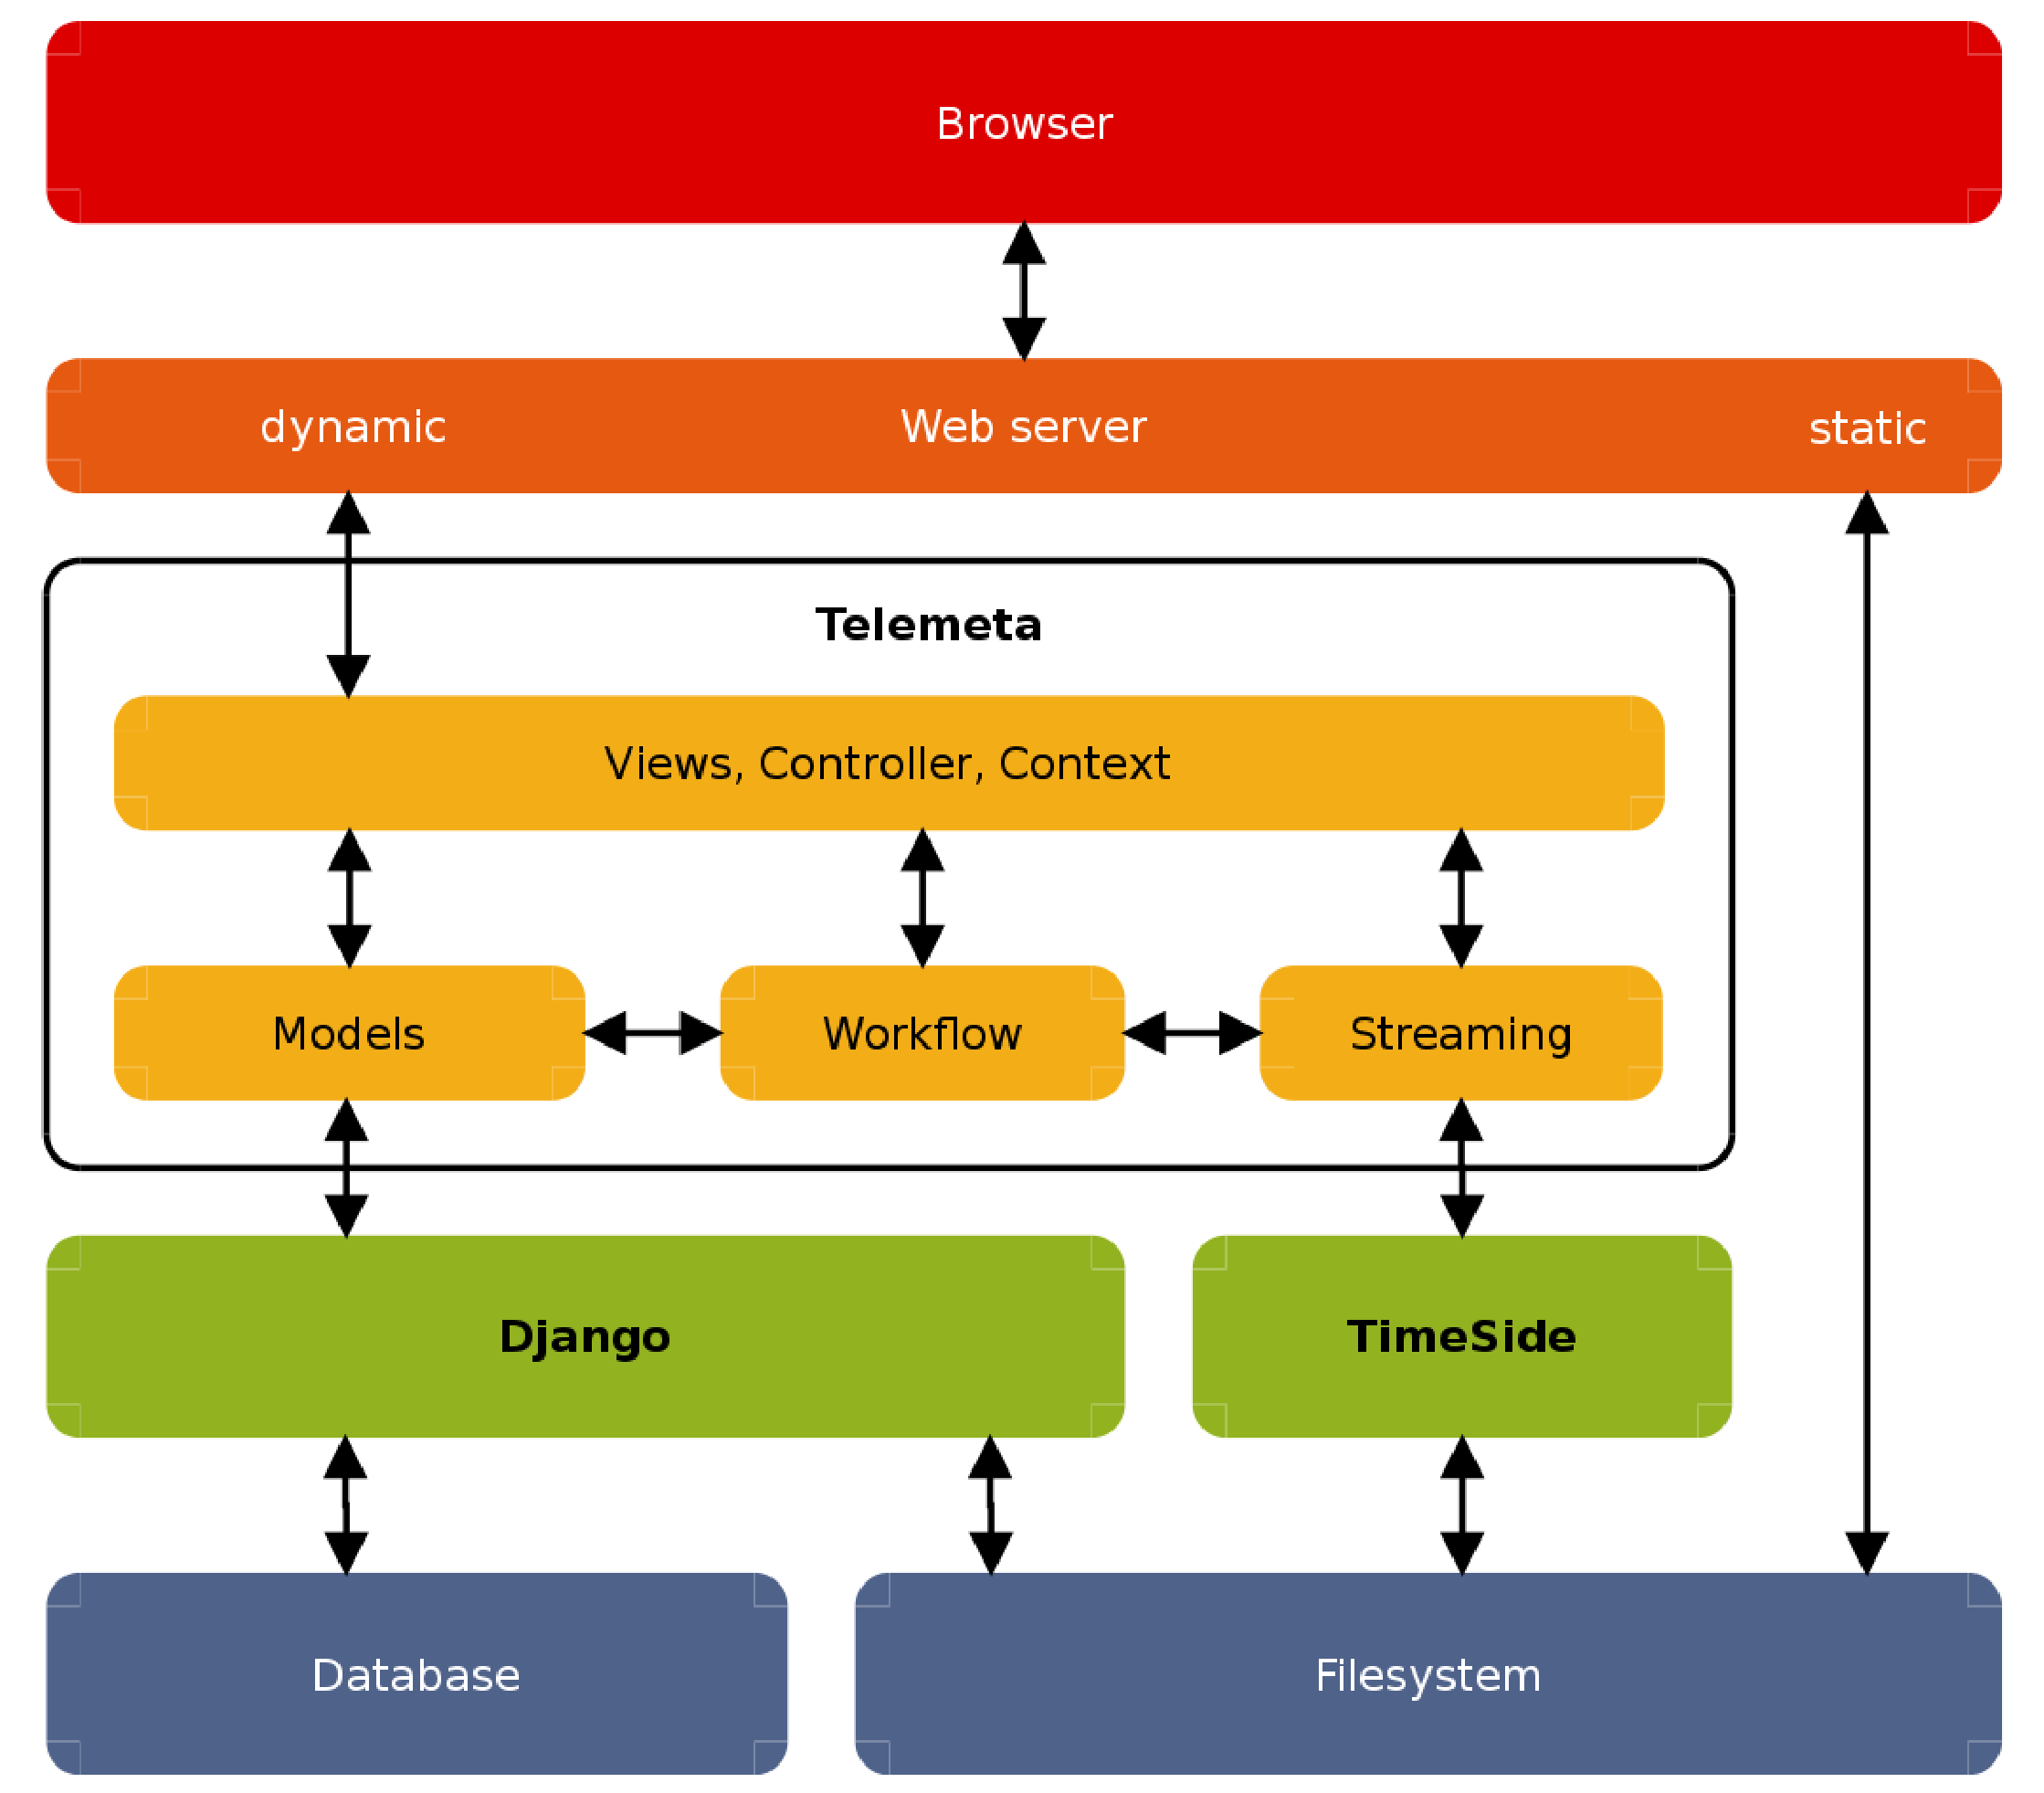
\includegraphics[width=0.9\linewidth]{img/TM_arch.pdf}
  \caption{Telemeta architecture}\label{fig:TM_arch}
  \label{fig:screenshot}
\end{figure}
The main features of \emph{Telemeta} are:
      \begin{itemize}
      \item Pure HTML5 web user interface including dynamical forms
      \item On-the-fly audio analyzing, transcoding and metadata
        embedding in various multimedia formats
      \item Social editing with semantic ontologies, smart workflows,
        realtime tools, human or automatic annotations and
        segmentations
      \item User management with individual desk, playlists, profiles
        and group access rights
      \item High level search engine (geolocation, instruments, ethnic groups, etc...)
      \item Data providers : DublinCore, OAI-PMH, RSS, XML, JSON and other 
      \item Multi-language support (now english and french)
      \end{itemize}
Beside database management, the audio support is mainly provided through an external component, TimeSide, which is described in Section~\ref{sec:TimeSide}.
\subsection{Metadata}\label{sec:metadata}
In addition to the audio data, an efficient and dynamic management of the associated metadata is also necessary. Consulting metadata grants both an exhaustive access to valuable information about the source of the data and to the related work of peer researchers. 
Dynamically handling metadata in a collaborative manner optimizes the continuous process of knowledge gathering and enrichment of the materials in the database.  
One of the major challenges is thus the standardization of audio and metadata formats with the aim of long-term preservation and usage of the different materials.
The compatibility with other systems is facilitated by the integration of the metadata standards protocols \emph{Dublin Core}\footnote{{Dublin Core} Metadata Initiative, \url{http://dublincore.org/}} and \emph{OAI-PMH} (Open Archives Initiative Protocol for Metadata Harvesting)\footnote{\url{http://www.openarchives.org/pmh/}}.
The metadata includes two different kinds of information about the audio item: contextual information and analytical information of the audio content.
\subsubsection{Contextual Information}
In an ethnomusicological framework, contextual information may include details about the location where the recording has been made, the instruments, the population, the title of the musical piece, the cultural elements related to the musical item, the depositor, the collector, the year of the recording and the year of the publication. 
Moreover, through the platform, diverse materials related to the archives can be stored, such as iconographies (digitalized pictures, scans of booklet and field notes, and so on), hyperlinks and biographical information about the collector. 

\subsubsection{Descriptive and analytical information on the audio content}
The second type of metadata consists in information about the audio content itself. This metadata can relate to the global content of the audio item or provide temporally-indexed information. It should also be noted that such information can be produced either by a human expert or by an automatic computational audio analysis (see Section~\ref{sec:TimeSide} below).

\squeezeup\paragraph{Visual representation and segmentation}
As illustrated in Figure~\ref{fig:sound_representation}, the TimeSide audio player embedded in the Telemeta web page view of a sound item allows for a selection of various visual representations of the sound (e.g. waveforms and spectrograms, see section~\ref{sec:TimeSide} for details) and some representations of computational analysis that can be combined with visual representations.
\begin{figure}[htb]
  \centering
  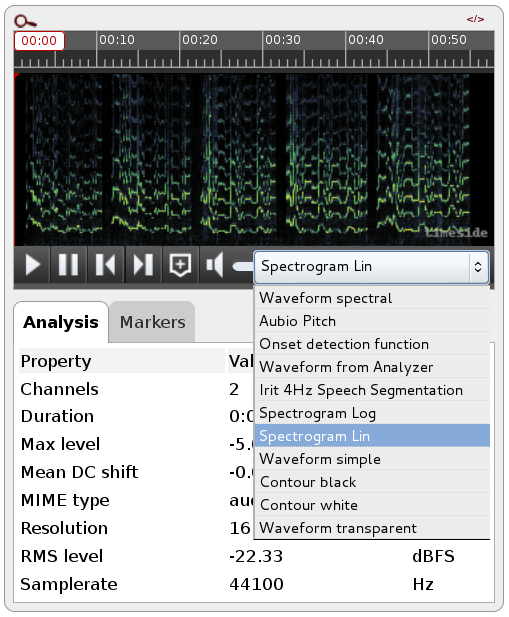
\includegraphics[width=0.5\linewidth]{img/sound_representation.png}
  \caption{Selection of various sound representation.}
  \label{fig:sound_representation}
\end{figure}
Among those automatic analysis some can produce a list of of time-segments associated with labels.
Those labels have been specified by the partners of the Diadems project (see Section~\ref{sec:Diadems} to be relevant for ethnomusicological studies (e.g. detection of spoken voice versus sang one, chorus, musical instrument categories, and so on).

\squeezeup\paragraph{Annotations}
As illustrated on Figure~\ref{fig:screenshot}, the embedded audio player also enables to annotate the audio content through time-coded markers.
Such annotations consist in a title and a free text field associated with a given time position.

Ethnomusicologists, archivists, as well as anthropologists, linguists and acousticians working on sound documents can create their own annotations and share them with colleagues. These annotations are accessible from the sound archive item web page and are indexed through the database.

It should be noted that the possibility for experts to annotate time-segments over a zoomable representation of the sound is currently under development in order to improve the accuracy and the quality of time-segment base annotations.


\section{TimeSide, an audio analysis framework}\label{sec:TimeSide}
One specificity of the Telemeta architecture is to rely on an external component, TimeSide\footnote{\url{https://github.com/yomguy/TimeSide}}, that offers audio player web integration together with audio signal processing analysis capabilities. 
TimeSide is an audio analysis and visualization framework based on both python and javascript languages to provide state-of-the-art signal processing and machine learning algorithms together with web audio capabilities for display and streaming.
Figure~\ref{fig:TimeSide_Archi} illustrates the overall architecture of TimeSide together with the data flow between TimeSide and the Telemeta web-server.
\begin{figure}[htbp]
  \centering
  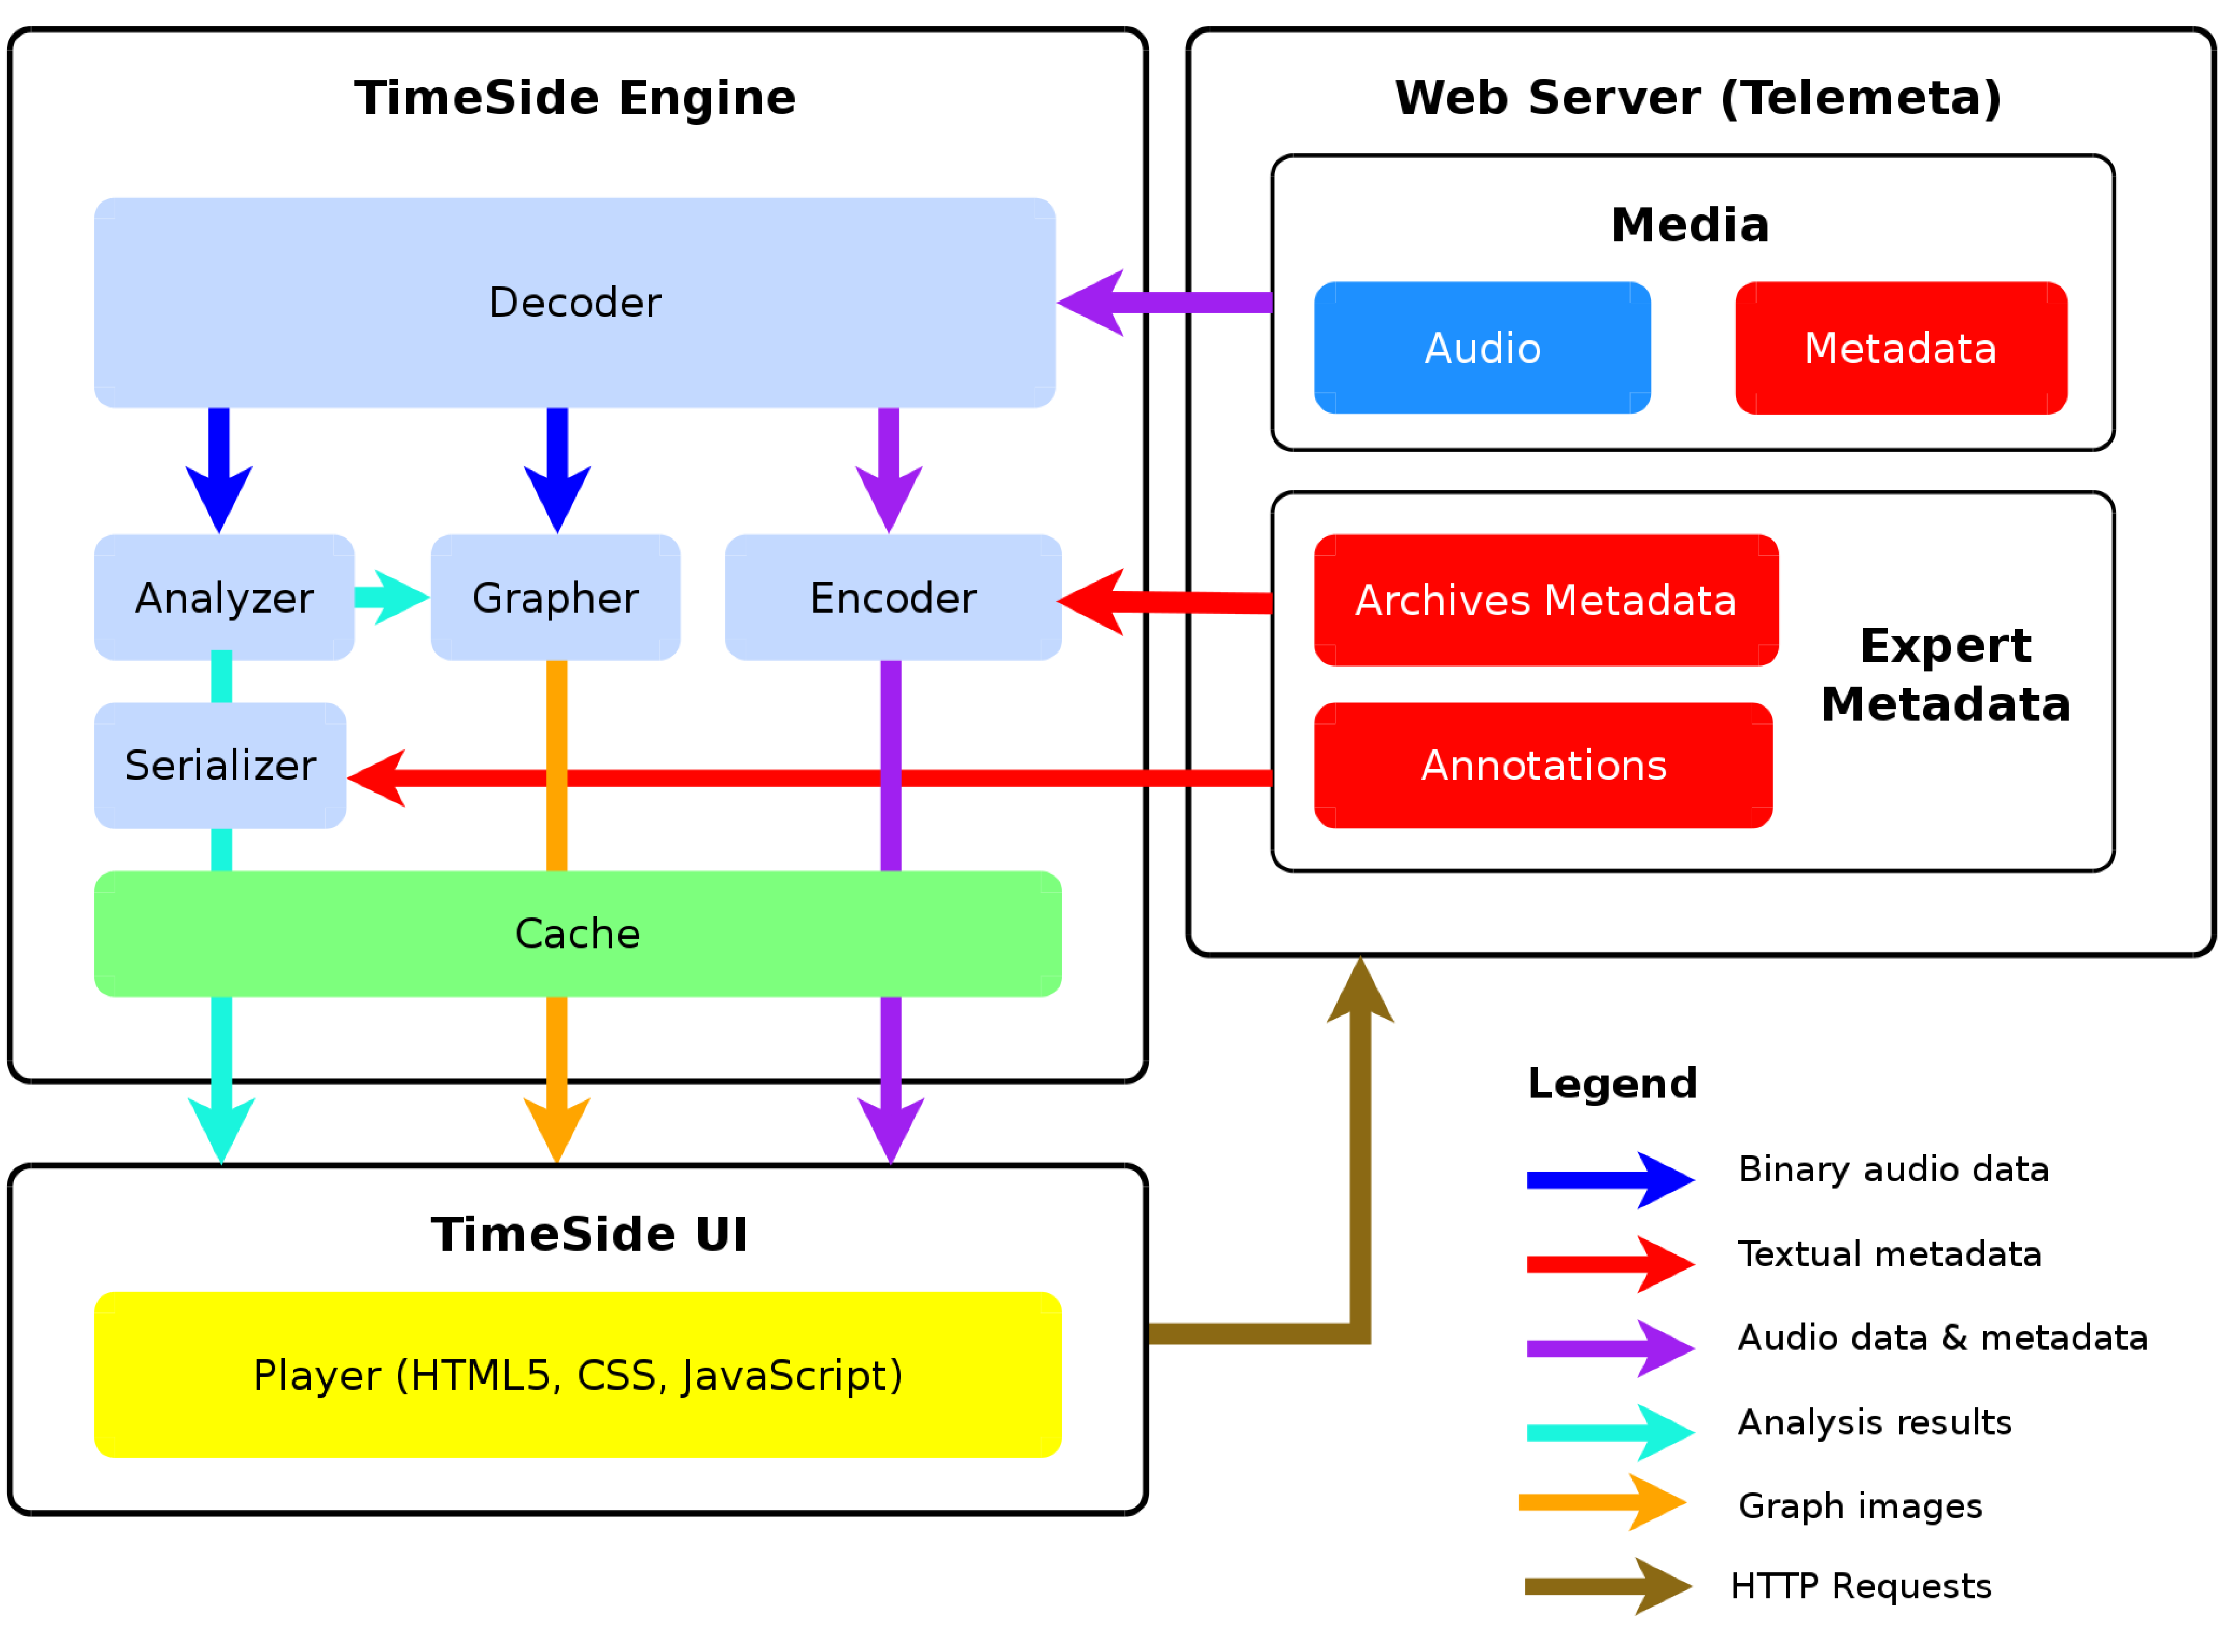
\includegraphics[width=\linewidth]{img/timeside_schema_v3.pdf}
  \caption{TimeSide engine architecture and data flow with Telemeta web-server}\label{fig:TimeSide_Archi}
\end{figure}

\subsection{Audio management}
TimeSide provides the following main features:
\begin{itemize}
\item Secure archiving, editing and publishing of audio files over
  internet.
\item Smart audio player with enhanced visualisation (waveform, spectrogram)
\item Multi-format support: reads all available audio and video formats  through Gstreamer, transcoding with smart streaming and caching methods% (FLAC, OGG, MP3, WAV and WebM)
  % \item \emph{Playlist management} for all users with CSV data export
\item On-the-fly audio analyzing, transcoding and metadata
    embedding based on an easy plugin architecture
\end{itemize}
\subsection{Audio features extraction}
In order to implement Music Information Retrieval analysis methods to be carried out over a large corpus for ethnomusicological studies, TimeSide incorporates some state-of-the-art audio feature extraction libraries such as Aubio\footnote{\url{http://aubio.org/}} \cite{brossierPhD}, Yaafe\footnote{\url{https://github.com/Yaafe/Yaafe}} \cite{yaafe_ISMIR2010} and Vamp plugins\footnote{ \url{http://www.vamp-plugins.org}}.
As a open-source framework and given its architecture and the flexibility provided by Python, the implementation of any audio and music analysis algorithm can be considered. Thus, it makes it a very convenient framework for researchers in computational ethnomusicology to develop and evaluate their algorithms.
Given the extracted features, every sound item in a given collection can be automatically analyzed. The results of this analysis can be stored in a scientific file format like Numpy and HDF5, exported to sound visualization and annotation softwares like sonic visualizer \cite{cannam2006sonic},or serialized to the web browser through common markup languages: XML, JSON and YAML.



\section{Sound archives of the \\CNRS - Musée de l'Homme}\label{sec:archives-CREM}
Since June 2011, the Telemeta platform is used by the  \emph{Sound archives of the CNRS - Musée de l'Homme}\footnote{\url{http://archives.crem-cnrs.fr}} and managed by the CREM (\CREM). According to the CREM specific aims, the Telemeta platform makes these archives available for researchers, students and, when copyright allows it, to a broader audience. Through this platform, these archives can be shared, discussed and worked on.

The Telemeta platform have also been deployed for the sound archives of the \emph{String instruments - Acoustic - Music} team of the ``Jean Le Rond d'Alembert Institute''\footnote{\url{http://telemeta.lam-ida.upmc.fr/}. Online since 2012, these archives consist in recordings of a wide range of musical instruments, mostly including solo recording of traditional instruments and illustrating various playing techniques and are used as materials for research in acoustics.}.



\subsection{Archiving research materials}
The Sound archives of the CNRS - Musée de l'Homme is one of the most important in Europe and gather commercial as well as unpublished recordings of music and oral traditions from around the world, collected by researchers attached to numerous research institutions across the world, among which some prominent figures of the field of ethnomusicology (among which Brailoiu, Lomax, Shaeffner, Rouget and Elkin). 

The platform offers access to records collection (nearly 3700 hours, e.g. more than 5000 discs, many of which are very rare) and to 4000 hours of unpublished recordings, as early expeditions (e.g. Dakar-Djibouti (1932), Ogooué-Congo (1946)). Most of the recordings comes from the fieldwork of researchers in all the continents. 
More than 110 years of the world's oral culture are now available online, from the 1900 Universal Exhibition of Paris up to the recent digital recordings. The sharing of data allows many people to collaborate to the enrichment of the database. Today, 47,200 items are in the database, and more than 26,000 sound files have been included (12 000 sounds on free access in Mai 2014). Recently, the CREM has decided to give full access to the records published by the CNRS-Musée de l’Homme (Chant du Monde/Harmonia Mundi)\footnote{\url{http://archives.crem-cnrs.fr/archives/fonds/CNRSMH_Editions/}} which distribution stopped ten years ago.
As a web platform, this tool is also a way to cross borders, to get local populations involved in their own cultural heritage and to offer resources to researchers from all over the world.

\subsection{Uses and users of digital sound archives}
     Through the few years since the sound archive platform had been released, it appears to support three main activities: archive, research and education (academic or not). These usages are those of archivists, researchers (ethnomusicologists, anthropologists and linguists), students and professors of these disciplines. Nonetheless, a qualitative survey showed that other disciplines (such as art history) found some use of the platform to foster and/or deepen individual research. The unexpectedly broad uses of the sound archives once digitalised and accessible emphasise the necessity and the benefits of such database.
From the standpoint of archive development, the long-term preservation of the archives is ensured while, thanks to the collaborative nature of the platform, users can cooperate to continuously enrich metadata associated with a sound document and submit their own archives to protect them. Furthermore, it allows fulfilling the ethical task of returning the recorded music to the communities who produced it.
Researchers from different institutions can work together on specific audio materials as well as conduct individual research in both synchronic and diachronic perspective, on their own material, others’ material or both.
When use for education, the platform provides a wide array of teaching material to illustrate students’ work as well as support teaching curricula.



\section{Expanding development: the DIADEMS project}\label{sec:Diadems}

The goals and expectations of the platform are of many kinds and expand through time, as users experience new ways to work with the archives database and request new tools to broaden the scope of their research activities linked to it. The reflexion collectively engaged by engineers and researchers on the use of the sound archives database led us  to set up a large scale project called DIADEMS (\emph{Description, Indexation, Access to Ethnomusicological and Sound Documents})\footnote{\url{http://www.irit.fr/recherches/SAMOVA/DIADEMS/en/welcome/}}. 
%DIADEMS is a French national research program, started in January 2013, with three IT research labs (IRIT\footnote{Institut de Recherche en Informatique de Toulouse}, , , LIMSI\footnote{Laboratoire d’Informatique pour la Mécanique et les Sciences de l’Ingénieur}, LABRI\footnote{Laboratoire Bordelais de Recherche en Informatique})\comment{TF: + LAM + labo ethno + Parisson. Plutôt dire a collaboration between ethno + IT}
Started in January 2013, the French national research program DIADEMS is a multi-disciplinary project whose consortium includes research laboratories from \emph{ Science and Technology of Information and Communication}\footnote{IRIT (Institute of research in computing science of Toulouse), LABRI (Bordeaux laboratory of research in computer science), LIMSI (Laboratory of computing and mechanics for engineering sciences), LAM (String instruments - Acoustic - Music, Jean Le Rond d'Alembert Institute)} domain, \emph{Musicology and Ethnomusicology}\footnote{LESC (Laboratory of Ethnology and Comparative Sociology), MNHN (National Museum of Natural History)} domain and Parisson, a company involved in the development of Telemeta.
 
The goal of Diadems project is to develop computer tools to automatically index the recording content directly from the audio signal in order to improve the access to and the indexation of this vast ethnomusicological archive. Numerous ethnomusicological recordings contain speech and other types of sounds that we categorized as sounds from the environment (such as rain, insect or animal sounds, engine noise and so on) and sounds generated by the recording (such as sound produced by the wind in the microphone or sounds resulting from the defect of the recording medium). The innovation of this project is to automatize the indexation of the audio recordings directly from the recorded sound itself. Ongoing works consist in implementing advanced classification, indexation, segmentation and similarity analysis methods dedicated to ethnomusicological sound archives.  Besides music analysis, such automatic tools also deal with speech and other types of sounds classification and segmentation to enable a most exhaustive annotation of the audio materials.

%The goal of Diadems project is to propose a set of tools for automatic analysis of audio documents which may contain fields recordings: speech, singing voice, instrumental music, technical noises, natural sounds, etc. The innovation is to automatize the indexation of  audio recordings directly from the audio signal itself, in order to improve the access and indexation of anthropological archives. Ongoing works consist in implementing advanced classification, segmentation and similarity analysis methods,  specially suitable to ethnomusicological sound archives. The aim is also to propose tools to analyse musical components and musical structure. 
Automatic analysis of ethnomusicological sound archives is considered as a challenging task.
Field recordings generally contain more sound sources, noise, and recording artefacts than those obtained in studio conditions.
Automatic analysis of these recordings requires methods having a stronger robustness.
Preliminary Implementations  of speech detection models, and speaker diarisation methods, based on  \cite{barras2006multistage} have been integrated to TimeSide. 
While these models are well suited to radio-news recordings, the current developpement tasks consist to adapt these methods to the particular case of ethnographic archives.

In the context of this project, researchers from Ethnomusicological, Speech and Music Information Retrieval(MIR) communities are working together to specify the tasks to be addressed by automatic analysis tools.


\subsection{The method of a new interdisciplinary research}

In this research program, groups from different backgrounds are working together to specify the automatic analysis tools :  IT developers, humanities researchers (anthropologists, ethnomusicologists, ethnolinguists) and specialists on speech and MIR. The first challenge was to initiate a common interest and a mutual understanding. In this process, DIADEMS gave us the opportunity  to improve our understanding on the link between the semantics and acoustics of voice production. As a prelimirary work we attempted to first define vocal categories with a particular interest for liminal oral productions. At the border between speech and song, utterances such as psalmody or recitation are at the center of an old debate in ethnomusicology\footnote{A colloquium on liminal utterances between speech and song will be organised by the International Council for Traditional Music (ICTM) in May 2015 and hosted by the Centre of research in Ethnomusicology (CREM). A round table will be dedicated to the presentation of the main results and findings of the ANR project Diadems}. Gathering specialists from various fields, Diadems project goes well beyond the usual disciplinary boundaries. Our aim, through the study of a large range of audio components (pitch range, syllabic flow, metric, polyphonic and so on) is to define and characterize the variability of vocal productions, keeping in mind the semantic aspects. By doing so, we wish to reduce the traditional gap in academic studies between sounds and semantics and to propose combined analytical tools for the study of vocal production\footnote{As an example, research will be conducted on the recognition of "icons of crying" 
in lamented utterances. As defined by Urban in \cite{Urban88}, "icons of crying" include cry break, voice inhalation, creaky voice and falsetto vowels.}. 

One of the goals of the DIADEMS project is also to provide also useful tools for musical analysis such as tools for detection of musical instrument families, analysis of musical content (tonal, metric and rythmic features), musical similarities and structure (chorus localisation, musical pattern replication).

The study follow three steps : 
\begin{enumerate}
\item The development of tools and selection of a representative corpus
  for each tool,
\item The evaluation of the proposed automatic analysis, in addition to
  the human-led evaluations carried on the corpus selected,
\item The development of a visual interface with an ergonomic access and
  import of the results in the database.
\end{enumerate}



\subsection{Automatic tools for assisting indexation and annotation of audio documents}
A first concern was to develop an automated annotation component that could differentiate spoken from sung voice and from instrumental music. If detection tools existed already to separate what is spoken from what is not, they were specifically designed to fit the needs of radio broadcast data (i.e. clear recordings produced in studios) and were not adapted to face the sonic diversity of ethnomusicological field recordings. For these, more refined detection tools were needed to pick up sound events such as overlapping speeches, speech over music, as well as instrumental music mixed with singing and/or spoken interventions.
Beyond the implementation of tools detecting the start and stop sound signatures of magnetic, mechanical and digital recorders as well as tape noises and silences, numerous algorithms allow for complex automated analysis for a wide range of combinations of vocal and instrumental sounds.


\subsubsection{Analysis of recordings sessions}
A primary concern of people dealing with audio materials coming from field recordings is to quickly and automatically identify the position of the start and stop time of the recording session.

In the case of digital recorder, the proposed system for localizing the start of recording sessions is based on the observation that on such recorders, the powering of the recorder implies a characteristic perturbation of the signal visible in Figure~\ref{plop}. This perturbation can be modeled by using the two different shapes of the temporal energy as references as the phenomenon appears to be quite reproducible over multiple recordings. On the analyzed recordings, the evolution of temporal energy of low energy segments is then compared to the models by an euclidean distance using the best alignment of the energy shape.

\begin{figure}[htb]
 \centering
    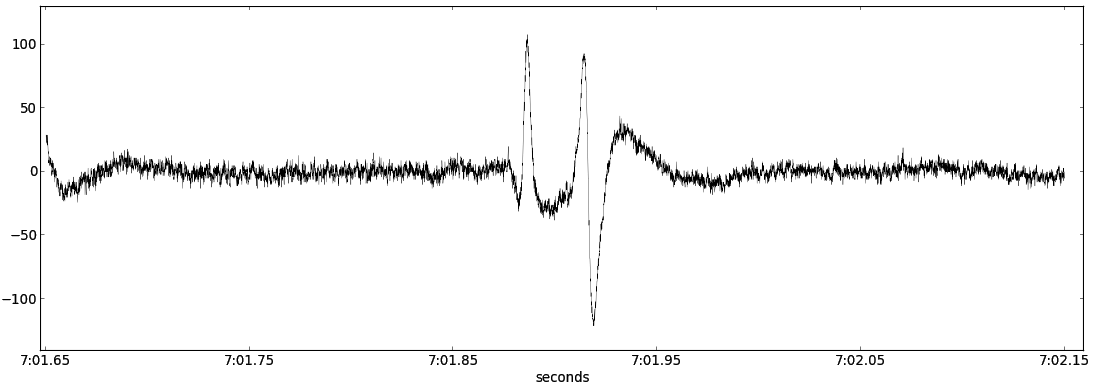
\includegraphics[width=0.8\linewidth]{img/plop.png}
    \caption{Typical perturbation produced by the recorder powering, used to recognise session start.}
    \label{plop}
\end{figure}


\subsubsection{Analysis of speech and singing voice segments}
Quick identification and localisation of spoken sections, particularly in rather long recordings, are relevant for all the disciplines involved in the project. The difficulties inherent in the sound materials led to the development of tools to automatically detect the occurrences of speech when performed simultaneously or alternatively with music; when numerous speakers interact and/or overlap with each others, with or without additional music or noises; and when voices modulate from speech to song, using a wide range of vocal techniques (recitation, narration, psalmody, back channel, and so on). The algorithms developed also allow for the analysis of the syllabic flow and the prosody of the speech. 
Figure~\ref{fig:speech_detection} shows a visual example of how speech segmentation is rendered.

%Source : CNRSMH_I_2013_201_001_01/
\begin{figure}[htb]
  \centering
 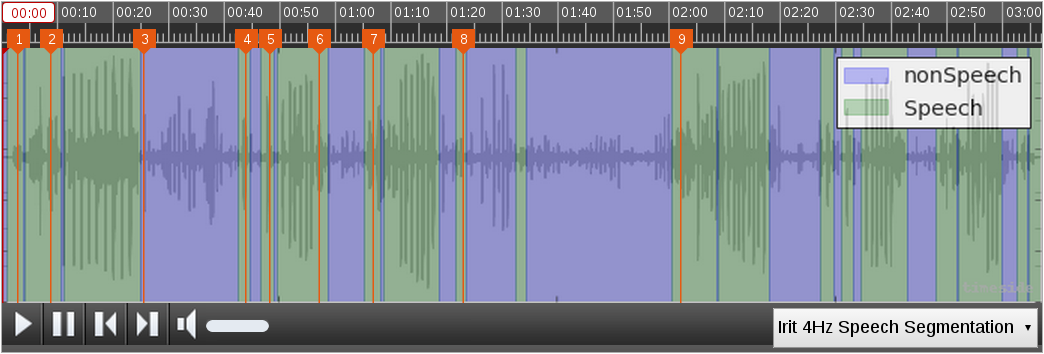
\includegraphics[width=\linewidth]{img/IRIT_Speech4Hz.png} 
  \caption{Detection of spoken voices in a song}
  \label{fig:speech_detection}
\end{figure}

\squeezeup\paragraph{Speech segmentation, with 2 features: 4 Hz modulation energy and entropy modulation} 
Speech signal has a characteristic energy modulation peak around the 4 Hertz syllabic rate \cite{Houtgast1985}. In order to model this property, the signal is filtered with a FIR band pass filter, centered on 4 Hertz.
Entropy modulation is dedicated to discriminate between speech and music~\cite{Pinquier2003}. We first evaluate the signal entropy ($H=\sum_{i=1}^{k}-p_ilog_2p_i$, with $p_i=$proba. of event~$i$). Entropy modulation values are usually larger for speech than for music. This measure is used to compute the entropy modulation on each segment. 

\squeezeup\paragraph{Speech activity detection based on GMM models}

The proposed method performs frame level speech activity detection based on a Gaussian Mixture Model (GMM). For each frame of the signal, the log likelihood difference between a speech model and a non speech model is computed.
The highest is the estimate, the largest is the probability that the frame corresponds to speech. 

For this task, a first reference model has been trained on data distributed during the ETAPE campaign\footnote{http://www.afcp-parole.org/etape.html}. A preliminary evaluation on a corpus collected by the French center of Research and teaching on Amerindian Ethnology (EREA) has been done and has demonstrated that this model was not appropriate for such a corpus containing a lot of background noise and Mayan language.
A second model have thus been trained on a this corpus and have provided better results.

\subsubsection{Analysis of music segments}
The DIADEMS project aims to provide useful tools for musical analysis in both research and teaching frameworks. To do so, it is also necessary to detect segments of instrumental music along with the recognition of the different musical instrument categories. Pushing the detection further into details, the tools implemented provide musicological information to support sound analysis (such as tonal, metric and rhythmic features) and allow for the detection of similarities in melody, harmony and rhythm as well as musical pattern replications.

\squeezeup\paragraph{Music segmentation, with 2 features based on a segmentation algorithm} 
This segmentation is provided by the Forward-Backward Divergence algorithm, which is based on a statistical study of the acoustic signal \cite{Obrecht1988}. The speech signal is assumed to be composed by a string of quasi-stationary units that can be seen as alternate periods of transient and steady parts (steady parts are mainly vowels). We characterize  each of these unites by an Auto Regressive (AR) Gaussian model. The method consists in performing a detection of changes in AR models. Indeed, music is usually much more constant than speech, that is to say the number of changes (segments) will be smaller for music than for speech. To estimate this, we count the number of segments per second of signal. The number of segments is the first discriminative feature for music segmentation.
The segments obtained with our segmentation algorithm  are generally longer for music than for speech. We chose to model the segment duration by a Gaussian Inverse law (Wald law) which is indeed our second feature providing a music segmentation.


\squeezeup\paragraph{Monophony / Polyphony segmentation}
A "monophonic" sound is defined as one note played at a time (either played by an instrument or sung by a singer), while a "polyphonic" sound is defined as several notes played simultaneously. The parameters extracted from the signal come from the YIN algorithm, a well known pitch estimator \cite{DeCheveigne2002}. Besides F0, this estimator provides an additional numerical value that can be interpreted as the inverse of a confidence indicator: the lower the value is, the more reliable the estimated pitch. Considering that when there is a single note the estimated pitch is fairly reliable, and that when there are several simultaneous notes, the estimated pitch is not reliable, we take the short term mean and variance of this "confidence indicator" as parameters for the monophony / polyphony segmentation. The bivariate distribution of these two parameters is modelled using Weibull bivariate distributions \cite{Lachambre2011}.
An example of the segmentation produced by this method is illustrated in Figure~\ref{fig:Monopoly}
% Source : CNRSMH_I_2000_008_001_04
\begin{figure}[htb]
  \centering
%\framebox[1.1\width]{Capture d'écran de IRIT Monopoly}
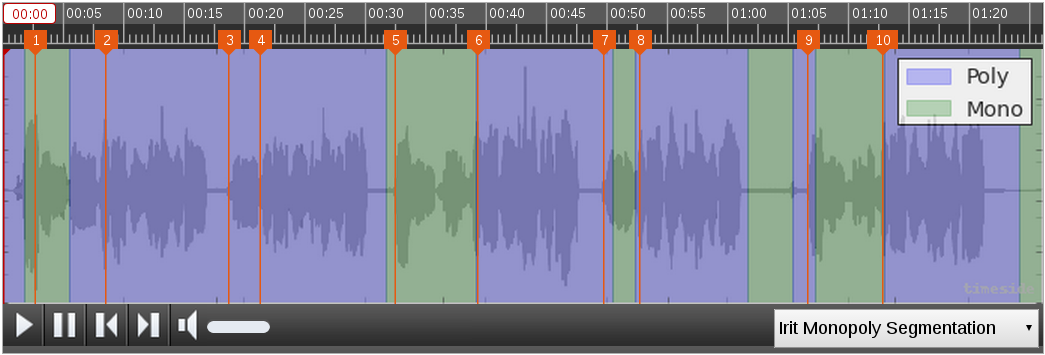
\includegraphics[width=0.95\linewidth]{img/SOLO_DUOdetection.png} 
 \caption{Detection solo and duo parts}
  \label{fig:Monopoly}
\end{figure}

\squeezeup\paragraph{Automatic instrument classification}
For the detection of musical instrument, we choose to follow the Hornbostel–Sachs system of musical instrument classification as first published in \cite{taxonomy_sachs2} and later translated in \cite{taxonomy_sachs}. This system is the most widely used system for classifying musical instruments by ethnomusicologists and organologists. together with more recent systems like the one proposed by Geneviève Dournon in \cite{Dournon92} and the \emph{RAMEAU} reference from the French national library (BnF)\footnote{\url{http://catalogue.bnf.fr/ark:/12148/cb119367821/PUBLIC}}.

We choose to develop tools to detect the four musical instrument families (cordophones, aerophones, idiophones, membranophones), but also refine subdivisions related to the playing techniques, identifying whether each instrument is blowed, bowed, plucked, struck or clincked by focusing on the 8 classes of instrument shown in Figure~\ref{fig:instruments}.

\begin{figure}[htb]
  \centering
  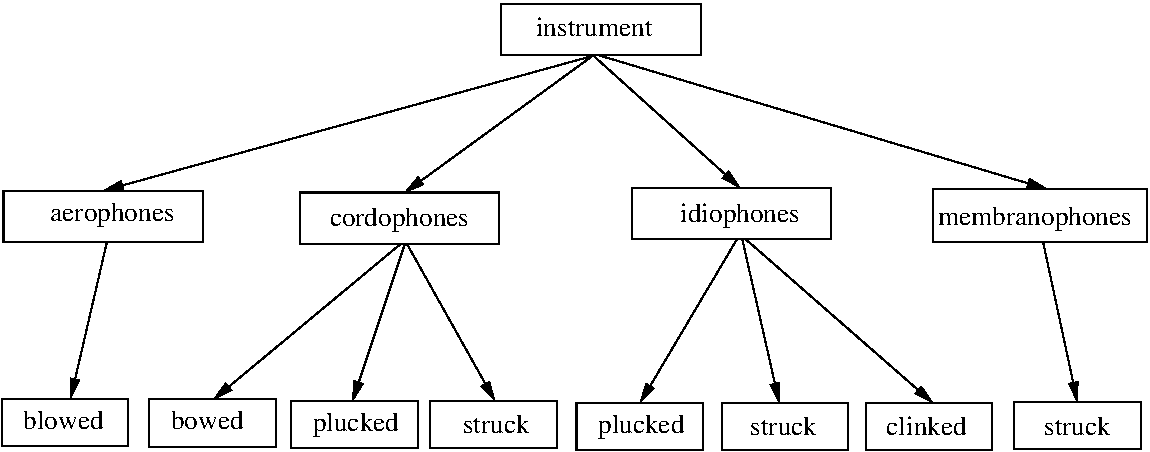
\includegraphics[width=0.9\linewidth]{img/taxonomie_diadems.pdf}
  \caption{Musical instrument families}
  \label{fig:instruments}
\end{figure}

The proposed method is based on the supervised learning approach and uses a set of 164 acoustic descriptors 
proposed by Peeters \textit{et al.} in \cite{timbre_toolbox}.
This system (see Figure~\ref{fig:inst_classif_method}) applies the Inertia Ratio Maximization Features Space (IRMFSP) algorihtm~\cite{aes_irmfsp} 
on annotated samples at the training step to reduce the number of features (to avoid overfitting) while selecting the most discriminative ones. %% see Figure 6

\begin{figure}[htb]
 \centering
 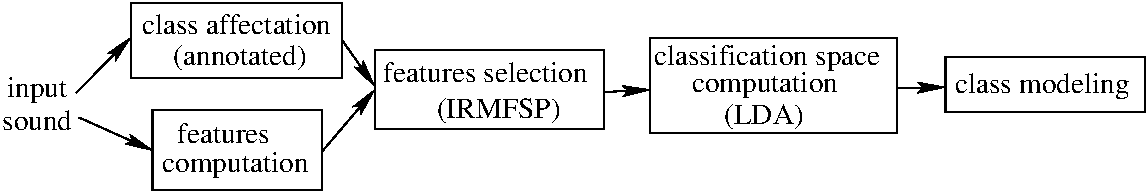
\includegraphics[width=0.9\linewidth]{img/method}
 \caption{Training step of the proposed classification method.}
 \label{fig:inst_classif_method}
\end{figure}

The Linear Discriminant Analysis (LDA) method~\cite{lda_book} is used to compute the best projection space 
or linear combination of all descriptors which maximizes the average distance between classes while minimizing the 
distance between individuals of the same class.

Each class is simply modeled into the classification space by its centroid (mean vector computed over the selected descriptors of the individuals which compose the class).
Thus, the classification task consists in projecting each tested sound described by a vector of descriptors
to the classification space and to select the closer class (in term of Euclidean distance to the class centroid). 

This simple and computationally efficient method obtains about 75\% of accuracy 
using the 20 most relevant descriptors projected on a 8-dimensions discriminative space. In a more detailed study~\cite{ismir14_dfourer},
this promising result was shown comparable with state-of-the art methods applied for the classification of western instruments recorded in studio condition.

% \begin{figure}[!ht]
%  \centering
% 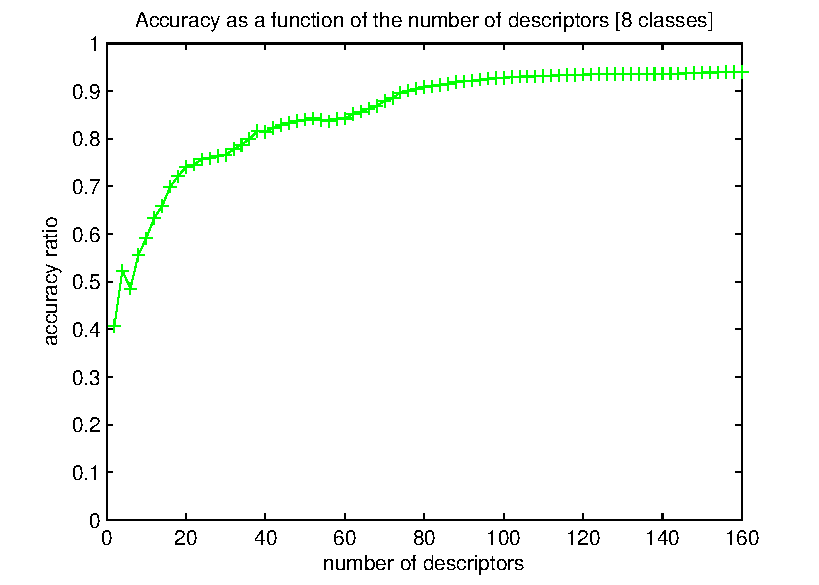
\includegraphics[width=0.7\linewidth]{img/crem_results}
%  \caption{3-fold cross-validation classification accuracy as a function of the number of optimally selected descriptors.}
%  \label{fig:inst_classif_result}
% \end{figure}


\subsection{Evaluation and sought improvements}

At the end of the first step of the project, interesting preliminary results have been obtained regarding sessions recordings, speech recognition, singing voice recognition and musical instrument family classification.

Through a collaborative work, ethnomusicologists, ethnolinguists and engineers are currently evaluating, correcting and refining the tools implemented, with the expectation that this work will lead to positive results, so these new tools can be integrated into the Telemeta platform. 

The robustness of all these processing are assessed using criteria defined by the final users: teachers, students, researchers or musicians. Annotation tools, as well as the provided annotations, will be integrated in the digitalized database. 

Further work on the user interface aims to enhance the visualization experience with time and frequency zooming capabilities, in the hope that it will improve the accuracy and the quality of time-segment based annotations. One of the remaining issues is to develop tools to generate results in line with the server processor and according to the capacities of Internet navigators while managing the workflow. 


\section{Conclusion}
 The Telemeta open-source framework provides researchers in humanities and social sciences with a new platform to efficiently distribute, share and work on their research on musical and sound materials. 
This platform offers automatic music analysis capabilities through the external component, TimeSide that provides a flexible computational analysis engine together with web serialization and visualization options. 
It brings an appropriate processing framework for researchers in computational ethnomusicology to develop and evaluate their algorithms. 
Deployed to manage the CNRS - Musée de l’Homme sound archives, the Telemeta platform has been conceived and adapted to generate tools in line with the needs of users. 

Thanks to the collaborative nature of the platform, users can continuously enrich metadata associated with sound archives. 

The benefits of this collaborative platform for the field of ethnomusicology apply to numerous aspects of research, ranging from musical analysis in a diachronic and synchronic comparative perspective, as well as the long-term preservation of sound archives and the support of teaching material for education. 


\section{Acknowledgments}
The authors would like to thank all the people that have been involved in Telemeta specification and development or have provide useful input and feedback. 
The project has been partially funded by the French National Centre for Scientific Research (CNRS), the French Ministry of Culture and Communication, the TGE Adonis Consortium, and the Centre of Research in Ethnomusicology (CREM).


\bibliographystyle{abbrv}
\bibliography{dlfm2014_Telemeta}

%\listofchanges

\end{document}
 
 
